\documentclass[aspectratio=169,11pt]{beamer}
\usepackage[T1]{fontenc}
\usepackage{lmodern,amsmath,amssymb,mathtools,bm,booktabs,array,graphicx,tikz}
\usetikzlibrary{arrows.meta,positioning,calc,decorations.pathreplacing,patterns}
\definecolor{ink}{HTML}{17344D}\definecolor{accent}{HTML}{087E8B}\definecolor{pale}{HTML}{EDF5F5}\definecolor{gold}{HTML}{AD6B19}
\providecommand{\dd}{\,\mathrm{d}}\providecommand{\R}{\mathbb{R}}
\providecommand{\E}{\mathbb{E}}\providecommand{\Var}{\operatorname{Var}}
\providecommand{\Cov}{\operatorname{Cov}}\providecommand{\diag}{\operatorname{diag}}
\providecommand{\norm}[1]{\left\lVert#1\right\rVert}
\providecommand{\abs}[1]{\left|#1\right|}
\usefonttheme{professionalfonts}
\setbeamercolor{normal text}{fg=black,bg=white}
\setbeamercolor{frametitle}{fg=ink,bg=white}
\setbeamercolor{title}{fg=ink}\setbeamercolor{structure}{fg=accent}
\setbeamercolor{block title}{fg=ink,bg=pale}\setbeamercolor{block body}{fg=black,bg=pale!40}
\setbeamercolor{alerted text}{fg=accent}
\setbeamerfont{frametitle}{size=\Large,series=\bfseries}
\setbeamerfont{title}{size=\LARGE,series=\bfseries}
\setbeamertemplate{navigation symbols}{}
\setbeamersize{text margin left=.7cm,text margin right=.7cm}
\setbeamertemplate{frametitle}{\vspace{.18cm}\insertframetitle\par\vspace{.1cm}{\color{accent}\hrule height .6pt}\vspace{.12cm}}
\newcommand{\notestarget}{notes.pdf}\newcommand{\noteslabel}{Notes}
\setbeamertemplate{footline}{\hspace{.7cm}\color{ink}\scriptsize Computational Cardiology\quad\href{\notestarget}{\noteslabel}\hfill\insertframenumber\,/\,\inserttotalframenumber\hspace{.7cm}\vspace{.18cm}}
\setbeamercovered{invisible}
\hypersetup{pdfauthor={Zan Ahmad},pdftitle={Fourier-mode error analysis of a transport discretization},pdfpagemode=UseNone}
\begin{document}
\begin{frame}[plain]\vfill
{\small\color{accent} Computational Cardiology \quad Lecture 6}\par\medskip
{\raggedright\hyphenpenalty=10000\exhyphenpenalty=10000\LARGE\bfseries\color{ink} Fourier-mode error analysis of a transport discretization}\par\bigskip
Zan Ahmad\par\smallskip
{\small Fall 2024}\par\vfill\end{frame}
\renewcommand{\notestarget}{notes.pdf\#note-an-exact-periodic-solution-and-its-cell-averages}
\begin{frame}[t,fragile,label=slide-a-continuum-transport-mode]{A continuum transport mode}
\[c(x,t)=1+A e^{-Dk^2t}\sin(k(x-at)),\qquad k=2\pi/L.\]\pause{} Advection changes phase; diffusion changes amplitude.
\end{frame}
\renewcommand{\notestarget}{notes.pdf\#note-an-exact-periodic-solution-and-its-cell-averages}
\begin{frame}[t,fragile,label=slide-differentiate-the-reference]{Differentiate the reference}
\[\partial_t c=-a\partial_x c+D\partial_{xx}c.\]\pause{} The sine satisfies periodic boundary conditions and retains mean one.
\end{frame}
\renewcommand{\notestarget}{notes.pdf\#note-an-exact-periodic-solution-and-its-cell-averages}
\begin{frame}[t,fragile,label=slide-match-the-represented-state]{Match the represented state}
\[\bar c_i=1+A\operatorname{sinc}(k\Delta x/2)e^{-Dk^2t}\sin(k(x_i-at)).\]\pause{} Here $\operatorname{sinc}z=\sin z/z$. Cell averages differ from midpoint samples.
\end{frame}
\renewcommand{\notestarget}{notes.pdf\#note-norms-and-observed-convergence-order}
\begin{frame}[t,fragile,label=slide-an-rms-error]{An RMS error}
\[E_h=\left(\frac1N\sum_i|\bar c_i^{\rm num}-\bar c_i^{\rm ref}|^2\right)^{1/2}.\]\pause{} All values refer to the same physical time and the same averaging convention.
\end{frame}
\renewcommand{\notestarget}{notes.pdf\#note-norms-and-observed-convergence-order}
\begin{frame}[t,fragile,label=slide-observed-order]{Observed order}
\[E_h\simeq Ch^p\quad\Longrightarrow\quad p_{\rm obs}=\log_2(E_h/E_{h/2}).\]\pause{} A slope requires an asymptotic regime; two nearly equal runs are not sufficient.
\end{frame}
\renewcommand{\notestarget}{notes.pdf\#note-the-symbol-of-the-spatial-operator}
\begin{frame}[t,fragile,label=slide-fourier-diagonalization]{Fourier diagonalization}
\[c_i=z e^{\mathrm i i\theta},\qquad c_{i\pm1}=e^{\pm\mathrm i\theta}c_i.\]\pause{} A translation-invariant stencil acts on this vector by multiplication.
\end{frame}
\renewcommand{\notestarget}{notes.pdf\#note-the-symbol-of-the-spatial-operator}
\begin{frame}[t,fragile,label=slide-the-spatial-eigenvalue]{The spatial eigenvalue}
\[\lambda_h=-\frac{|a|}{\Delta x}(1-\cos\theta)-\frac{4D}{\Delta x^2}\sin^2(\theta/2)-\mathrm i\frac a{\Delta x}\sin\theta.\]\pause{} Its real part damps the mode; its imaginary part transports its phase.
\end{frame}
\renewcommand{\notestarget}{notes.pdf\#note-the-symbol-of-the-spatial-operator}
\begin{frame}[t,fragile,label=slide-the-leading-spatial-error]{The leading spatial error}
\[\lambda_h=-\mathrm iak-Dk^2-\frac{|a|k^2}{2}\Delta x+O(\Delta x^2).\]\pause{} Upwind advection is first order. Pure centered diffusion removes the $O(\Delta x)$ term.
\end{frame}
\renewcommand{\notestarget}{notes.pdf\#note-the-symbol-of-the-spatial-operator}
\begin{frame}[label=slide-exact-semi-discrete-evolution-panel-1]{Space: time error removed}
\centering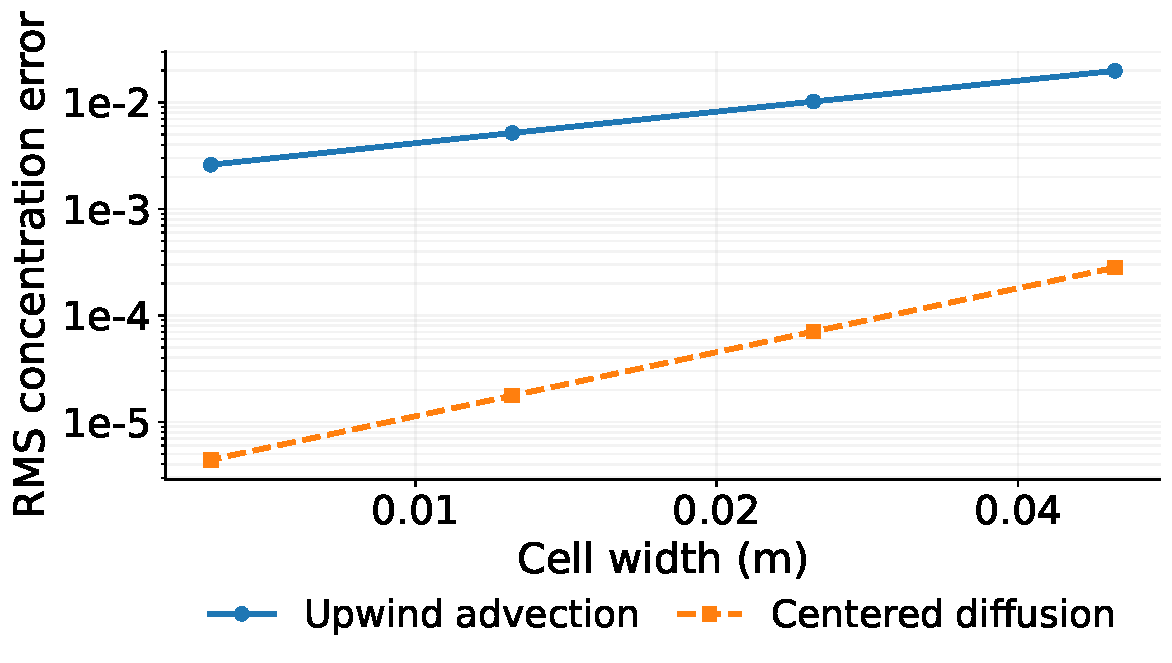
\includegraphics[width=.98\linewidth,height=.69\textheight,keepaspectratio]{presentation-figures/separate-errors-panel-1.pdf}\end{frame}
\renewcommand{\notestarget}{notes.pdf\#note-the-symbol-of-the-spatial-operator}
\begin{frame}[label=slide-exact-semi-discrete-evolution-panel-2]{Time: Euler at fixed grid}
\centering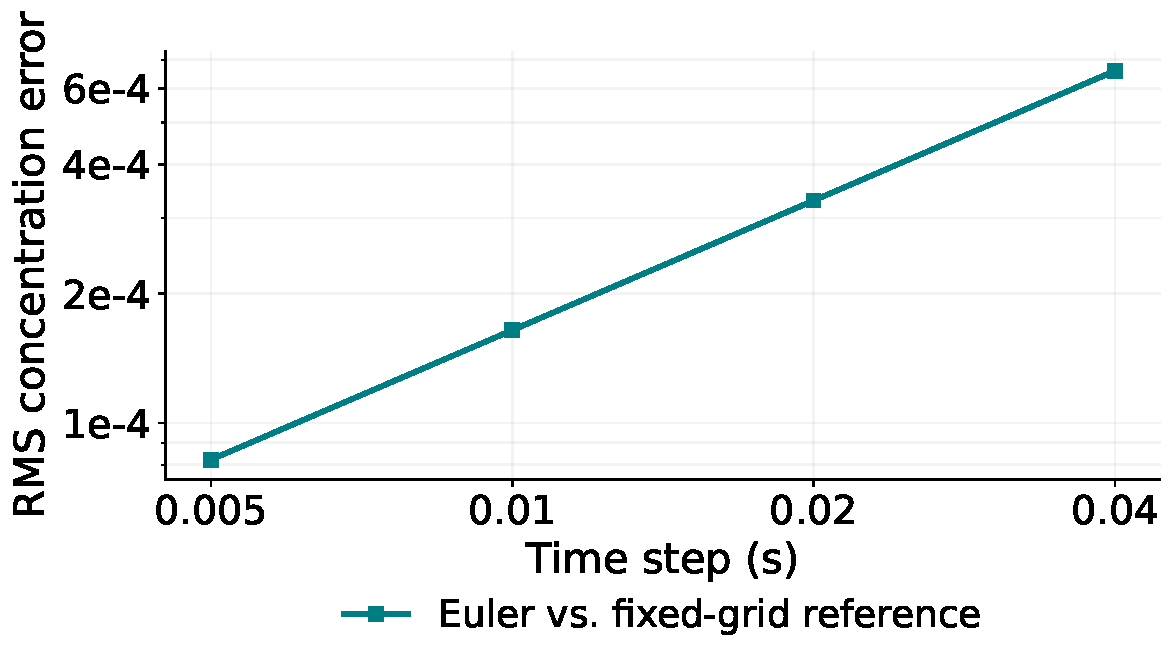
\includegraphics[width=.98\linewidth,height=.69\textheight,keepaspectratio]{presentation-figures/separate-errors-panel-2.pdf}\end{frame}
\renewcommand{\notestarget}{notes.pdf\#note-the-symbol-of-the-spatial-operator}
\begin{frame}[t,fragile,label=slide-exact-semi-discrete-evolution]{Exact semi-discrete evolution}
\[z(t)=e^{\lambda_h t}z(0).\]\pause{} Compare this with the continuum mode to isolate spatial error.
\end{frame}
\renewcommand{\notestarget}{notes.pdf\#note-separate-space-and-time-refinement}
\begin{frame}[t,fragile,label=slide-euler-amplification-at-a-fixed-grid]{Euler amplification at a fixed grid}
\[z^{n+1}=(1+\Delta t\lambda_h)z^n.\]\pause{} Compare $(1+\Delta t\lambda_h)^{T/\Delta t}$ with $e^{T\lambda_h}$ to isolate time error.
\end{frame}
\renewcommand{\notestarget}{notes.pdf\#note-separate-space-and-time-refinement}
\begin{frame}[t,fragile,label=slide-accumulated-temporal-error]{Accumulated temporal error}
\[\frac{T}{\Delta t}\log(1+\Delta t\lambda_h)=T\lambda_h-\frac{T\Delta t}2\lambda_h^2+O(\Delta t^2).\]\pause{} The leading difference is first order in $\Delta t$.
\end{frame}
\renewcommand{\notestarget}{notes.pdf\#note-the-highest-frequency-diffusion-mode}
\begin{frame}[t,fragile,label=slide-a-grid-scale-perturbation]{A grid-scale perturbation}
\[c_i=1+\varepsilon(-1)^i,\qquad\theta=\pi.\]\pause{} On an even periodic grid the perturbation sums to zero.
\end{frame}
\renewcommand{\notestarget}{notes.pdf\#note-the-highest-frequency-diffusion-mode}
\begin{frame}[label=slide-diffusive-amplification-figure]{Unstable diffusion steps amplify noise}
\centering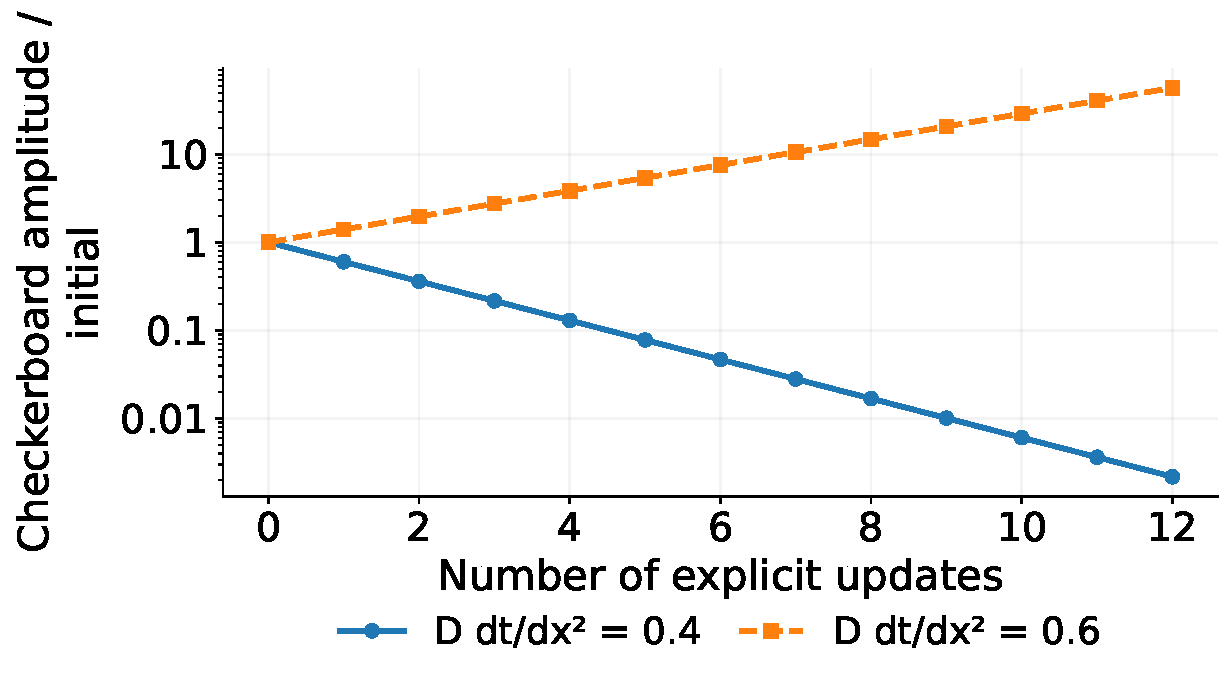
\includegraphics[width=.98\linewidth,height=.69\textheight,keepaspectratio]{presentation-figures/stability-mode-panel-1.pdf}\end{frame}
\renewcommand{\notestarget}{notes.pdf\#note-the-highest-frequency-diffusion-mode}
\begin{frame}[t,fragile,label=slide-diffusive-amplification]{Diffusive amplification}
\[\varepsilon^{n+1}=(1-4\mu)\varepsilon^n.\]\pause{} For $\mu=.4$ the factor is $-.6$; for $\mu=.6$ it is $-1.4$.
\end{frame}
\renewcommand{\notestarget}{notes.pdf\#note-the-highest-frequency-diffusion-mode}
\begin{frame}[t,fragile,label=slide-conservation-is-compatible-with-instability]{Conservation is compatible with instability}
The alternating mode remains mean-zero while its magnitude grows.\pause{}\[|1-4\mu|\le1\quad\Longleftrightarrow\quad0\le\mu\le\tfrac12.\]
\end{frame}
\renewcommand{\notestarget}{notes.pdf\#note-limits-of-the-single-mode-analysis}
\begin{frame}[t,fragile,label=slide-the-scope-of-fourier-analysis]{The scope of Fourier analysis}
Constant coefficients and periodic translations make the modes independent.\pause{} A boundary, variable coefficient or nonlinear reaction introduces additional structure that this calculation does not analyze.
\end{frame}
\end{document}
